% Drawing 115/01-1 -- folder 115, batch 01, archive page 2 (PDF page 3).
% Transcription: le reste de la page, tenue tête-bêche, barré de deux longs traits obliques : une roue de huit catégories de foncteurs ($\underline{\mathrm{Hom}}(A^{\wedge}, B^{\wedge})$ et ses variantes) reliées par des flèches le long d'un cercle, premier état de la roue de la page 5 ; au-dessous, un graphe de triangles aux sommets marqués $A^{\wedge}$, $B^{\wedge}$ et variantes.
% Kind: wheel of functor categories and a graph of triangles, wholly struck. Method 2 (schematic redraw from the facsimile). Status: partial.
% Notes: Earlier record (2026-11-12, 2026-11-13, #128, #147): an empty redraw of a struck sketch, put to the editor on /review/. Redrawn 2026-11-14 per #154: the editor (Michel) asked for the figure to be redrawn although it is struck, « it's interesting », and noted that the sheet is upside down. The sheet is a printer listing used tete-beche: the crop is turned 180 degrees and the figure drawn the right way up, coordinates in the turned crop. Everything is drawn in the struck style (grey), as for 45 04-1 and 91 02-1; the two long oblique strokes that cross it out are not drawn. Drawn: above the wheel once the sheet is turned (« au-dessous » in the transcription, which follows the sheet as filed), the graph of triangles: the quadrilateral A^,B^v -- A^,B^ -- A^v,B^ -- A^v,B^v with its edge labels A^ (ink), B^, B^v (pencil), A^v (ink), and the pencil strokes going up from its vertices to the two labels A^°--B^ and B^°--A^ and to a point at the upper right (three verticals, four obliques). Below, the wheel: a pencil circle, eight functor categories round it (top Hom^!(A^°,B^), then clockwise Hom^!!_!(A^°,B^v;Ens), Hom_!(B^v,A^), Hom_!!(A^v,B^v;Ens), Hom_!(A^v,B^), Hom^!!_!!(A^v,B^v;Ens) with « (…, 20, 22) » under it, Hom^!(B^°,A^), Hom^!!_!(A^°,B^v°;Ens)), the eight ink arrows along the circle (the one from Hom^!(B^°,A^) up to Hom^!!_!(A^°,B^v°;Ens) heavy), four pencil chords through the centre (A x B)^ joining opposite categories, and the labels of their halves: A^ and A^v on the vertical, B^ and B^v on the horizontal, ^v and v^ on the chord from upper right to lower left. Readings: the decorations ! and !! above and below Hom and the degree marks ° are read on the 400 dpi colour scan and are uncertain where he overinked them (top right and bottom left); A^ is written A^{wedge}, A^v A^{vee}, as in the transcription's description. Left out: the two small struck labels on the chord from upper left to lower right (scribbled over, a Hom with ^^ and with vv), the first number of « (…, 20, 22) » (overwritten, 44 or 42), and, outside the wheel, the note {A,B} x {^,v}, (A,v) x (^,v) at the right, which is writing. Overlay: the strokes rasterised over the 400 dpi colour crop lie on their ink to within about 1 unit (the pencil circle, slightly flattened at the lower left, is followed as a closed curve); the labels are set in print at their places. Partial because the labels are a reading of small, partly overinked writing. Not checked by a reader; not compiled (no TeX in the session).
% Coordinates: 1 unit = 1 mm = 1/100 of the crop width (bbox in page fractions: [0.1, 0.17, 0.54, 0.5]).
% Redrawn by Claude (claude-opus-5-5), issue #154, 2026-11-14 (vectorise-drawings); not checked by a human; not compiled (no TeX in the session).
% Rights: reproduces part of the work -- behind RENDER_TRANSCRIPTS, never published by itself.
\documentclass[tikz,border=3pt]{standalone}
\usepackage{amsmath,amssymb}
\usetikzlibrary{patterns,arrows.meta}
\tikzset{pencil/.style={black!45}, struck/.style={black!35}, mark/.style={circle,draw,inner sep=1.3pt}, pt/.style={circle,fill,inner sep=0.9pt}, opt/.style={circle,draw,fill=white,inner sep=1.1pt}}
\begin{document}
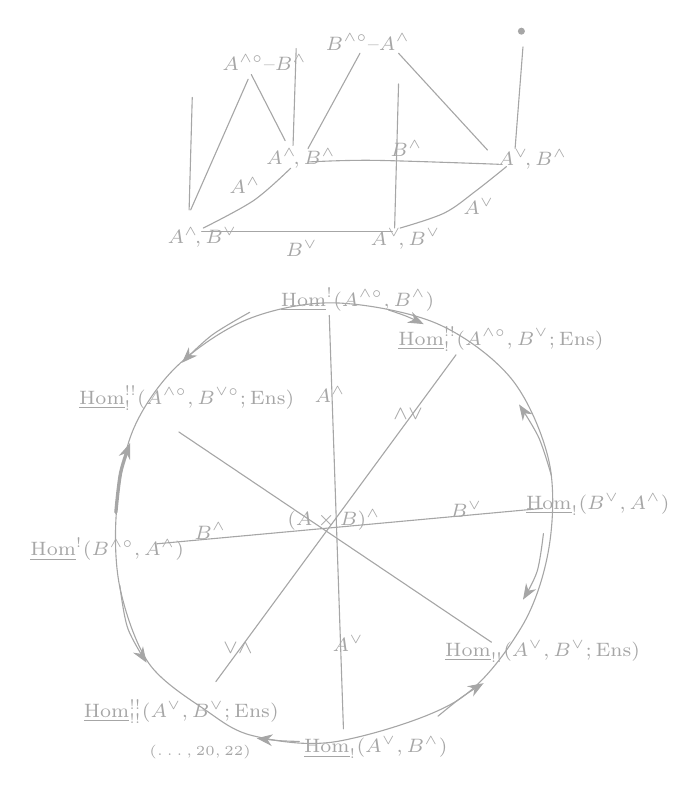
\begin{tikzpicture}[x=1mm,y=1mm,line cap=round,line join=round,font=\scriptsize]
\draw[struck] (29.1,-13.5) -- (21.8,-30.1);
\draw[struck] (29.5,-12.9) -- (33.8,-21.3);
\draw[struck] (22,-15.8) -- (21.6,-30.1);
\draw[struck] (35.2,-9.6) -- (34.8,-21.9);
\draw[struck] (43.3,-10.2) -- (36.7,-22.3);
\draw[struck] (48.2,-10.2) -- (59.5,-22.5);
\draw[struck] (48.2,-14.1) -- (47.7,-32.4);
\draw[struck] (64,-9.4) -- (63,-22.3);
\node[pt,struck] at (63.8,-7.4) {};
\draw[struck] plot[smooth, tension=0.55] coordinates {(23.4,-32.4) (29.8,-28.9) (34.5,-24.8)};
\draw[struck] plot[smooth, tension=0.55] coordinates {(36.9,-24) (45,-23.8) (60.9,-24.3)};
\draw[struck] (23.2,-32.8) -- (47.4,-32.8);
\draw[struck] plot[smooth, tension=0.55] coordinates {(48.4,-32.4) (54,-30.5) (58,-27.7) (61.9,-24.6)};
\node[inner sep=1pt,struck] at (31.2,-11.4) {\scriptsize $A^{\wedge\circ}\text{--}B^{\wedge}$};
\node[inner sep=1pt,struck] at (44.3,-8.8) {\scriptsize $B^{\wedge\circ}\text{--}A^{\wedge}$};
\node[inner sep=1pt,struck] at (23.3,-33.6) {\scriptsize $A^{\wedge}\!,B^{\vee}$};
\node[inner sep=1pt,struck] at (35.8,-23.6) {\scriptsize $A^{\wedge}\!,B^{\wedge}$};
\node[inner sep=1pt,struck] at (65.2,-23.7) {\scriptsize $A^{\vee}\!,B^{\wedge}$};
\node[inner sep=1pt,struck] at (49.1,-33.8) {\scriptsize $A^{\vee}\!,B^{\vee}$};
\node[inner sep=1pt,struck] at (28.7,-27) {\scriptsize $A^{\wedge}$};
\node[inner sep=1pt,struck] at (49.2,-22.3) {\scriptsize $B^{\wedge}$};
\node[inner sep=1pt,struck] at (35.9,-35) {\scriptsize $B^{\vee}$};
\node[inner sep=1pt,struck] at (58.4,-29.7) {\scriptsize $A^{\vee}$};
\draw[struck] plot[smooth cycle, tension=0.55] coordinates {(40,-41.9) (53,-44.5) (62.5,-51.5) (67.3,-62) (67.3,-73) (63.8,-83.1) (55.5,-92.5) (40.4,-97.6) (29.8,-96.9) (23.8,-93.7) (16.5,-87.7) (12.8,-78) (12.4,-68) (14.5,-58) (20,-50) (29,-44)};
\draw[struck] (39.4,-43.5) -- (41.2,-96);
\draw[struck] (17.5,-72.5) -- (66.5,-68);
\draw[struck] (55.5,-48.5) -- (25,-90);
\draw[struck] (20.3,-58.3) -- (60,-85);
\node[inner sep=1pt,struck] at (43,-41.5) {\scriptsize $\underline{\mathrm{Hom}}^{!}(A^{\wedge\circ},B^{\wedge})$};
\node[inner sep=1pt,struck] at (61.2,-46.5) {\scriptsize $\underline{\mathrm{Hom}}^{!!}_{!}(A^{\wedge\circ},B^{\vee};\mathrm{Ens})$};
\node[inner sep=1pt,struck] at (73.5,-67.5) {\scriptsize $\underline{\mathrm{Hom}}_{!}(B^{\vee},A^{\wedge})$};
\node[inner sep=1pt,struck] at (66.5,-86.2) {\scriptsize $\underline{\mathrm{Hom}}_{!!}(A^{\vee},B^{\vee};\mathrm{Ens})$};
\node[inner sep=1pt,struck] at (45.3,-98.4) {\scriptsize $\underline{\mathrm{Hom}}_{!}(A^{\vee},B^{\wedge})$};
\node[inner sep=1pt,struck] at (20.6,-93.8) {\scriptsize $\underline{\mathrm{Hom}}^{!!}_{!!}(A^{\vee},B^{\vee};\mathrm{Ens})$};
\node[inner sep=1pt,struck] at (23,-99) {\tiny $(\ldots,20,22)$};
\node[inner sep=1pt,struck] at (11.2,-73.2) {\scriptsize $\underline{\mathrm{Hom}}^{!}(B^{\wedge\circ},A^{\wedge})$};
\node[inner sep=1pt,struck] at (21.3,-54) {\scriptsize $\underline{\mathrm{Hom}}^{!!}_{!}(A^{\wedge\circ},B^{\vee\circ};\mathrm{Ens})$};
\draw[struck,-{Stealth[length=2mm]}] plot[smooth, tension=0.55] coordinates {(29.3,-43.1) (24.5,-46) (20.7,-49.5)};
\draw[struck,-{Stealth[length=2mm]}] plot[smooth, tension=0.55] coordinates {(46.9,-42.8) (49.2,-43.6) (51.4,-44.6)};
\draw[struck,-{Stealth[length=2mm]},very thick] plot[smooth, tension=0.55] coordinates {(12.3,-68.5) (12.9,-63.5) (14.1,-59.7)};
\draw[struck,-{Stealth[length=2mm]}] plot[smooth, tension=0.55] coordinates {(67.6,-63.8) (66,-59) (63.5,-54.8)};
\draw[struck,-{Stealth[length=2mm]}] plot[smooth, tension=0.55] coordinates {(66.6,-71.2) (65.8,-76) (64,-79.6)};
\draw[struck,-{Stealth[length=2mm]}] plot[smooth, tension=0.55] coordinates {(53.2,-94.4) (56.2,-92) (59,-90.2)};
\draw[struck,-{Stealth[length=2mm]}] plot[smooth, tension=0.55] coordinates {(35.6,-97.6) (33,-97.5) (30.2,-97.2)};
\draw[struck,-{Stealth[length=2mm]}] plot[smooth, tension=0.55] coordinates {(12.8,-77.8) (13.8,-83.2) (16.2,-87.6)};
\node[inner sep=1pt,struck] at (39.5,-53.6) {\scriptsize $A^{\wedge}$};
\node[inner sep=1pt,struck] at (49.4,-56) {\scriptsize ${\wedge}{\vee}$};
\node[inner sep=1pt,struck] at (40,-69.5) {\scriptsize $(A\times B)^{\wedge}$};
\node[inner sep=1pt,struck] at (24.3,-70.9) {\scriptsize $B^{\wedge}$};
\node[inner sep=1pt,struck] at (56.8,-68.2) {\scriptsize $B^{\vee}$};
\node[inner sep=1pt,struck] at (27.8,-85.8) {\scriptsize ${\vee}{\wedge}$};
\node[inner sep=1pt,struck] at (41.8,-85.2) {\scriptsize $A^{\vee}$};
\end{tikzpicture}
\end{document}
